%-------------------------------------------------------------------------------
% French version
%-------------------------------------------------------------------------------
\selectlanguage{french}
\chapter*[Introduction]{Introduction}
\addcontentsline{toc}{chapter}{Introduction (français)}
% Change numbering for introduction
\renewcommand{\thefigure}{\arabic{figure}}


L'humanité s'est toujours intéressée à la prédiction du temps pour le lendemain,
ainsi qu'à des échelles de temps plus longues. Depuis le milieu du
20\textsuperscript{eme} siècle, des modèles numériques ont été utilisés et
continuent d'être développés afin de prédire l'évolution de l'ensemble des
composantes de l'atmosphère. Ces modèles se divisent en deux catégories selon
l'échelle de temps considérée. Les modèles de climat globaux permettent de
prédire l'état moyen de l'atmosphère sur de longues périodes de temps, de
l'ordre de plusieurs années ou plus. Ils fonctionnent à l'échelle
globale, par opposition à l'échelle régionale, et nécessitent donc une
résolution plus grossière. Comme ils peuvent être utilisés pour estimer le
réchauffement climatique sur une période d'un siècle, leur coût informatique est
très élevé.  La seconde catégorie comporte les modèles de prévision
météorologique, qui sont ce qu'on associe en général avec la "météo".  Ces
modèles visent l'échelle régionale avec une échéance temporelle plus réduite, de
quelques heures à quelques jours. Ici, la précision et la rapidité d'exécution
sont des facteurs déterminants.  Cependant, la frontière entre ces deux
catégories est en train de s'estomper: les modèles globaux utilisent des
résolutions de plus en plus fines alors que les modèles régionaux augmentent la
taille de leur domaines. Comme ces modèles sont très complexes, ils sont divisés
en "blocs" dans la pratique, où chaque bloc gère un sous-ensemble de processus
physiques. Pour cette thèse, nous nous concentrons sur un de ces \DIFdelbegin \DIFdel{sous-modèles}\DIFdelend \DIFaddbegin \DIFadd{sous-ensembles}\DIFaddend ,
le modèle de chimie-transport (MCT).

Un modèle de chimie-transport modélise la chimie de l'atmosphère. Il s'agit
d'une tâche ardue par le nombre de processus, comme le montre la
Fig.~\ref{fig:atmospheric_proc}. Dans un modèle de la physique et chimie de
l'atmosphère, on se concentre généralement sur les processus principaux décrit
dans la Fig.~\ref{fig:chem_processes}, qui contribuent à l'évolution spatiale et
temporelle des espèces chimiques atmosphériques. Les modèles de chimie-transport
ont différentes applications, telles que l'estimation de l'impact des émissions
anthropiques. Lorsque des polluants sont émis en Asie, comme ce fut le cas
lors de l'incident à la centrale de Fukushima Daiichi, il peut être vital de
modéliser le transport au dessus de l'océan Pacifique. Les MCTs peuvent aussi
être utilisés pour étudier les cycles biochimiques comme la création ou le
transport des particules de sulfate lors d'éruptions volcaniques, comme ce fut
le cas avec l'Eyjafjallaj\"okull. Ces modèles peuvent aussi servir à établir des
simulation "paléochimiques" de la qualité de l'air à des époques préhistoriques
pour évaluer l'impact d'évènements extrêmes (tels que les impacts d'astéroïdes ou
les éruptions volcaniques) sur la chimie et le climat. Un autre champ
d'application est la prévision du "temps chimique", où la composition de
l'atmosphère est estimée sur plusieurs jours en utilisant des prévisions
météorologiques ainsi que des cadastres d'émissions. Dans ce cas, on se
concentre sur la couche limite, la stratosphère et la troposphère. Cela permet
de prédire l'indice d'UV ou les pics de pollution. Plusieurs pays en Europe ont
mis en place de tels systèmes. En France, le gouvernement a installé le projet
"Prév'air" pour permettre au grand public d'accéder à des prévisions de qualité
de l'air jusqu'à deux jours à l'aide des modèles MOCAGE et CHIMERE.  Les
résultats sont visible sur Internet (\url{www2.prevair.org}). Les MCTs
permettent également d'étudier les interactions entre la chimie et le changement
climatique. Ainsi, l'IGAC est un comité qui étudie entre autres l'impact de
l'ozone sur le changement climatique et les effets des aérosols sur les nuages
(\cite{IGAC2006}).

Pour cette thèse, nous nous focalisons sur les schémas numériques d'advection et
de chimie d'un MCT. En particulier, le but \DIFdelbegin \DIFdel{n'est pas }\DIFdelend \DIFaddbegin \DIFadd{de la thèse est }\DIFaddend de développer \DIFdelbegin \DIFdel{un c\oe{}ur
dynamique, qui contient d'autres processus que le transport, mais de se concentrer }\DIFdelend \DIFaddbegin \DIFadd{la
base d'un futur MCT en se concentrant }\DIFaddend sur l'advection de traceurs impliqués dans
la chimie atmosphérique.  Le développement de méthodes numériques pour le
transport est un domaine de recherche amorcé dans les années 60 et qui demeure
très actif aujourd'hui. Il y a principalement deux axes de recherche: le premier
étudie les méthodes numériques, le second se concentre sur l'adaptation de ces
méthodes aux coordonnées sphériques, qui possèdent certaines spécificités. La
grille régulière latitude-longitude est traditionnellement utilisée mais cette
grille a l'inconvénient d'avoir deux points singuliers (les pôles) ainsi qu'une
convergence des méridiens aux pôles. Cela impacte fortement les performances
informatiques et a conduit récemment à étudier des grilles alternatives.  Dans
l'état actuel, trouver une combinaison parfaite entre le schéma d'advection et
la grille sous-jacente reste un problème ouvert. \\ 
La chimie atmosphérique met en jeu des dizaines de milliers d'espèces chimiques.
Comme inclure dans un modèle numérique toutes ces espèces serait trop coûteux,
on se restreint en pratique à une centaine d'espèces. D'un point de vue
mathématique, il faut résoudre un système d'équations dit \textit{raide},
c'est-à-dire que les méthodes explicites sont inefficaces. De plus, la chimie
est locale contrairement à l'advection, donc en pratique cela justifie de
traiter la chimie et l'advection séparément dans un MCT.

Le choix d'un modèle dépend fortement de l'architecture informatique sur
laquelle il s'exécute. Alors que les modèles mathématiques existent depuis le
début du 20\textsuperscript{eme} siècle, les premiers modèles opérationnels de
prévisions mé\-téo\-ro\-lo\-gi\-que sont apparus dans les années 50.
L'augmentation de la puissance de calcul a conduit à une complexification des
modèles ainsi qu'à l'utilisation de résolutions de plus en plus fines. Cela a en
retour imposé une forte contrainte sur les performances des modèles.
L'augmentation de la résolution permet d'améliorer la précision à la fois de
l'advection et de la chimie, ce qui est notamment utile pour les MCGs, qui
visent maintenant une échelle régionale. De plus, les modèles de prévisions
météorologiques nécessitent que le modèle soit suffisamment rapide pour pouvoir
être intégré plusieurs fois par jour. Deux révolutions informatiques ont permis cette
course à la performance. La première fut l'avènement des machines vectorielles,
qui ont été depuis remplacées par des clusters de processeurs pouvant comporter
plusieurs centaines de milliers de c\oe{}urs. Dans le contexte actuel,
l'utilisation de ces processeurs multi-c\oe{}urs a aussi changé profondément la
manière dont sont envisagées les performances en parallèle. On privilégie
actuellement le passage à l'échelle des applications, c'est-à-dire l'utilisation
efficace d'un nombre très important et toujours croissant de c\oe{}urs.

\subsection*{Motivation}
Les schémas d'advection dans les modèles opérationnels actuels peuvent être
divisés en deux caté\DIFdelbegin \DIFdel{gories}\DIFdelend \DIFaddbegin \DIFadd{go-ries}\DIFaddend . En premier lieu, on peut regrouper les modèles
efficaces numériquement mais qui ne préservent pas la masse de manière
intrinsèque: ce sont les schémas de type semi-Lagrangiens. Ils sont efficaces
notamment parce qu'ils permettent des pas de temps plus longs que les schémas
Eulériens. Pour assurer que la masse est bien conservée de manière globale, des
correctifs \textit{a posteriori} sont en général appliqués. Cependant, la
conservation n'est pas assurée localement et ces correctifs ont un coût
numérique, qui impactera probablement les performances en parallèle. Dans la
seconde catégorie, on trouve les schémas conservatifs en point de grille,
principalement de type volumes-finis. Leur efficacité est cependant limitée par le
problème "des pôles" mentionné précédemment, qui diminue fortement le pas de
temps.

Cette thèse vise à résoudre ces deux problèmatiques en même temps en fournissant
un \DIFdelbegin \DIFdel{MCT }\DIFdelend \DIFaddbegin \DIFadd{modèle d'advection-chimie }\DIFaddend conservatif et efficace. De plus, nous imposons que
le modèle dispose d'une implantation parallèle performante et qui anticipe les
développements futurs des architectures parallèles, principalement en diminuant
le coût mémoire du modèle. Nous visons également à \DIFaddbegin \DIFadd{utiliser efficacement les
architectures parallèles de Météo-France. De plus, le but à moyen terme est de
créer un MCT complet afin de }\DIFaddend fournir une alternative à MOCAGE, le MCT de
Météo-France, ainsi qu'à \DIFdelbegin \DIFdel{utiliser efficacement les architectures parallèles de
Météo-France}\DIFdelend . C'est pourquoi ce manuscrit présente Pangolin (en
anglais \textit{a PArallel implementatioN of a larGe scale multi-dimensiOnaL
\DIFdelbegin \DIFdel{model}\DIFdelend \DIFaddbegin \DIFadd{chemIstry-traNsport scheme}\DIFaddend }), une infrastructure parallèle et efficace
pour l'advection et la chimie atmosphérique.


\subsection*{Plan}
\begin{itemize}
  \item Le chapitre~\ref{chap:transport} offre un aperçu des différents schémas
  d'advection et introduit le schéma en volumes-finis choisi pour Pangolin. Dans
  une seconde partie, nous étudions les différentes grilles disponibles sur la
  sphère. Puis, nous introduisons une nouvelle grille préservant
  approximativement les aires des cellules qui supprime le problème "des pôles".
  L'implantation du schéma volumes-finis sur cette grille est également
  détaillée.
  \item Le chapitre~\ref{chap:testing} examine les performances du schéma
  d'advection 2D sur des cas tests analytiques. Pangolin est aussi comparé à
  d'autres schémas de transport à l'aide d'une suite de tests récemment publiée.
  \item Le chapitre~\ref{chap:parallel} présente la stratégie utilisée pour
  paralléliser le modèle, avec notamment un algorithme de décomposition de
  domaine spécifiquement adapté à notre grille afin d'avoir une parallélisation
  efficace dans un contexte d'échange de messages. Les performances en
  parallèles pour l'advection 2D sont ensuite validées. Enfin, l'impact de la
  future chimie est estimé et nous discutons des différentes stratégies pour
  résoudre les problèmes qui en découlent.
  \item Le chapitre~\ref{chap:real_case} compare les résultats de Pangolin en 2D
    en coordonnées isentropiques à ceux de MOCAGE en 3D sur une simulation de
  distribution de l'ozone stratosphérique sur un mois. Le même schéma
  linéaire d'ozone est utilisé dans les deux modèles pour que la comparaison
  soit opportune.
\end{itemize}

\selectlanguage{english}

%-------------------------------------------------------------------------------
% English version
%-------------------------------------------------------------------------------

\chapter*[Introduction]{Introduction}
\addcontentsline{toc}{chapter}{Introduction}

\subsection*{Context}
Humans have always been interesting in predicting the weather, either for
tomorrow or for longer timescales. Since the middle of the 20th century,
numerical models are being used and under constant development to forecast the
state of the atmosphere. They currently fall into two categories, depending on
the time-scale. \glspl{GCM} aims at predicting the average state of the atmosphere
over large time periods, on the order of several years or more. They focus on
the global scale, as opposed to the regional scale, and use in practice a
coarser space resolution. As they can be used for example to estimate global
warming over a century, they are computationally expensive. On the
other hand, \glspl{NWP} is what the general public associates with "weather
prediction". It focuses on the regional scale with a smaller time-scale,
usually hourly to weekly. Accuracy and speed are the prime factors.
However, the boundary between these categories is beginning to blur as global
models are using finer resolutions and regional models are using a larger scale.
These models are also extremely complex so in practice, they are divided in
"blocks", where each block manages a smaller set of physical processes. In this
thesis, we focus on one of these \DIFdelbegin \DIFdel{submodels}\DIFdelend \DIFaddbegin \DIFadd{subset}\DIFaddend , the \gls{CTM}.

A CTM focuses on modelling the chemistry of the atmosphere. It is a complex task
with many processes, as illustrated by the Fig.~\ref{fig:atmospheric_proc}. On
Fig.~\ref{fig:chem_processes} are presented the main processes that should
appear in a physico-chemistry model of the atmosphere, which contribute to the
spatial and temporal evolution of the atmospheric species.
\begin{figure}
  \centering
  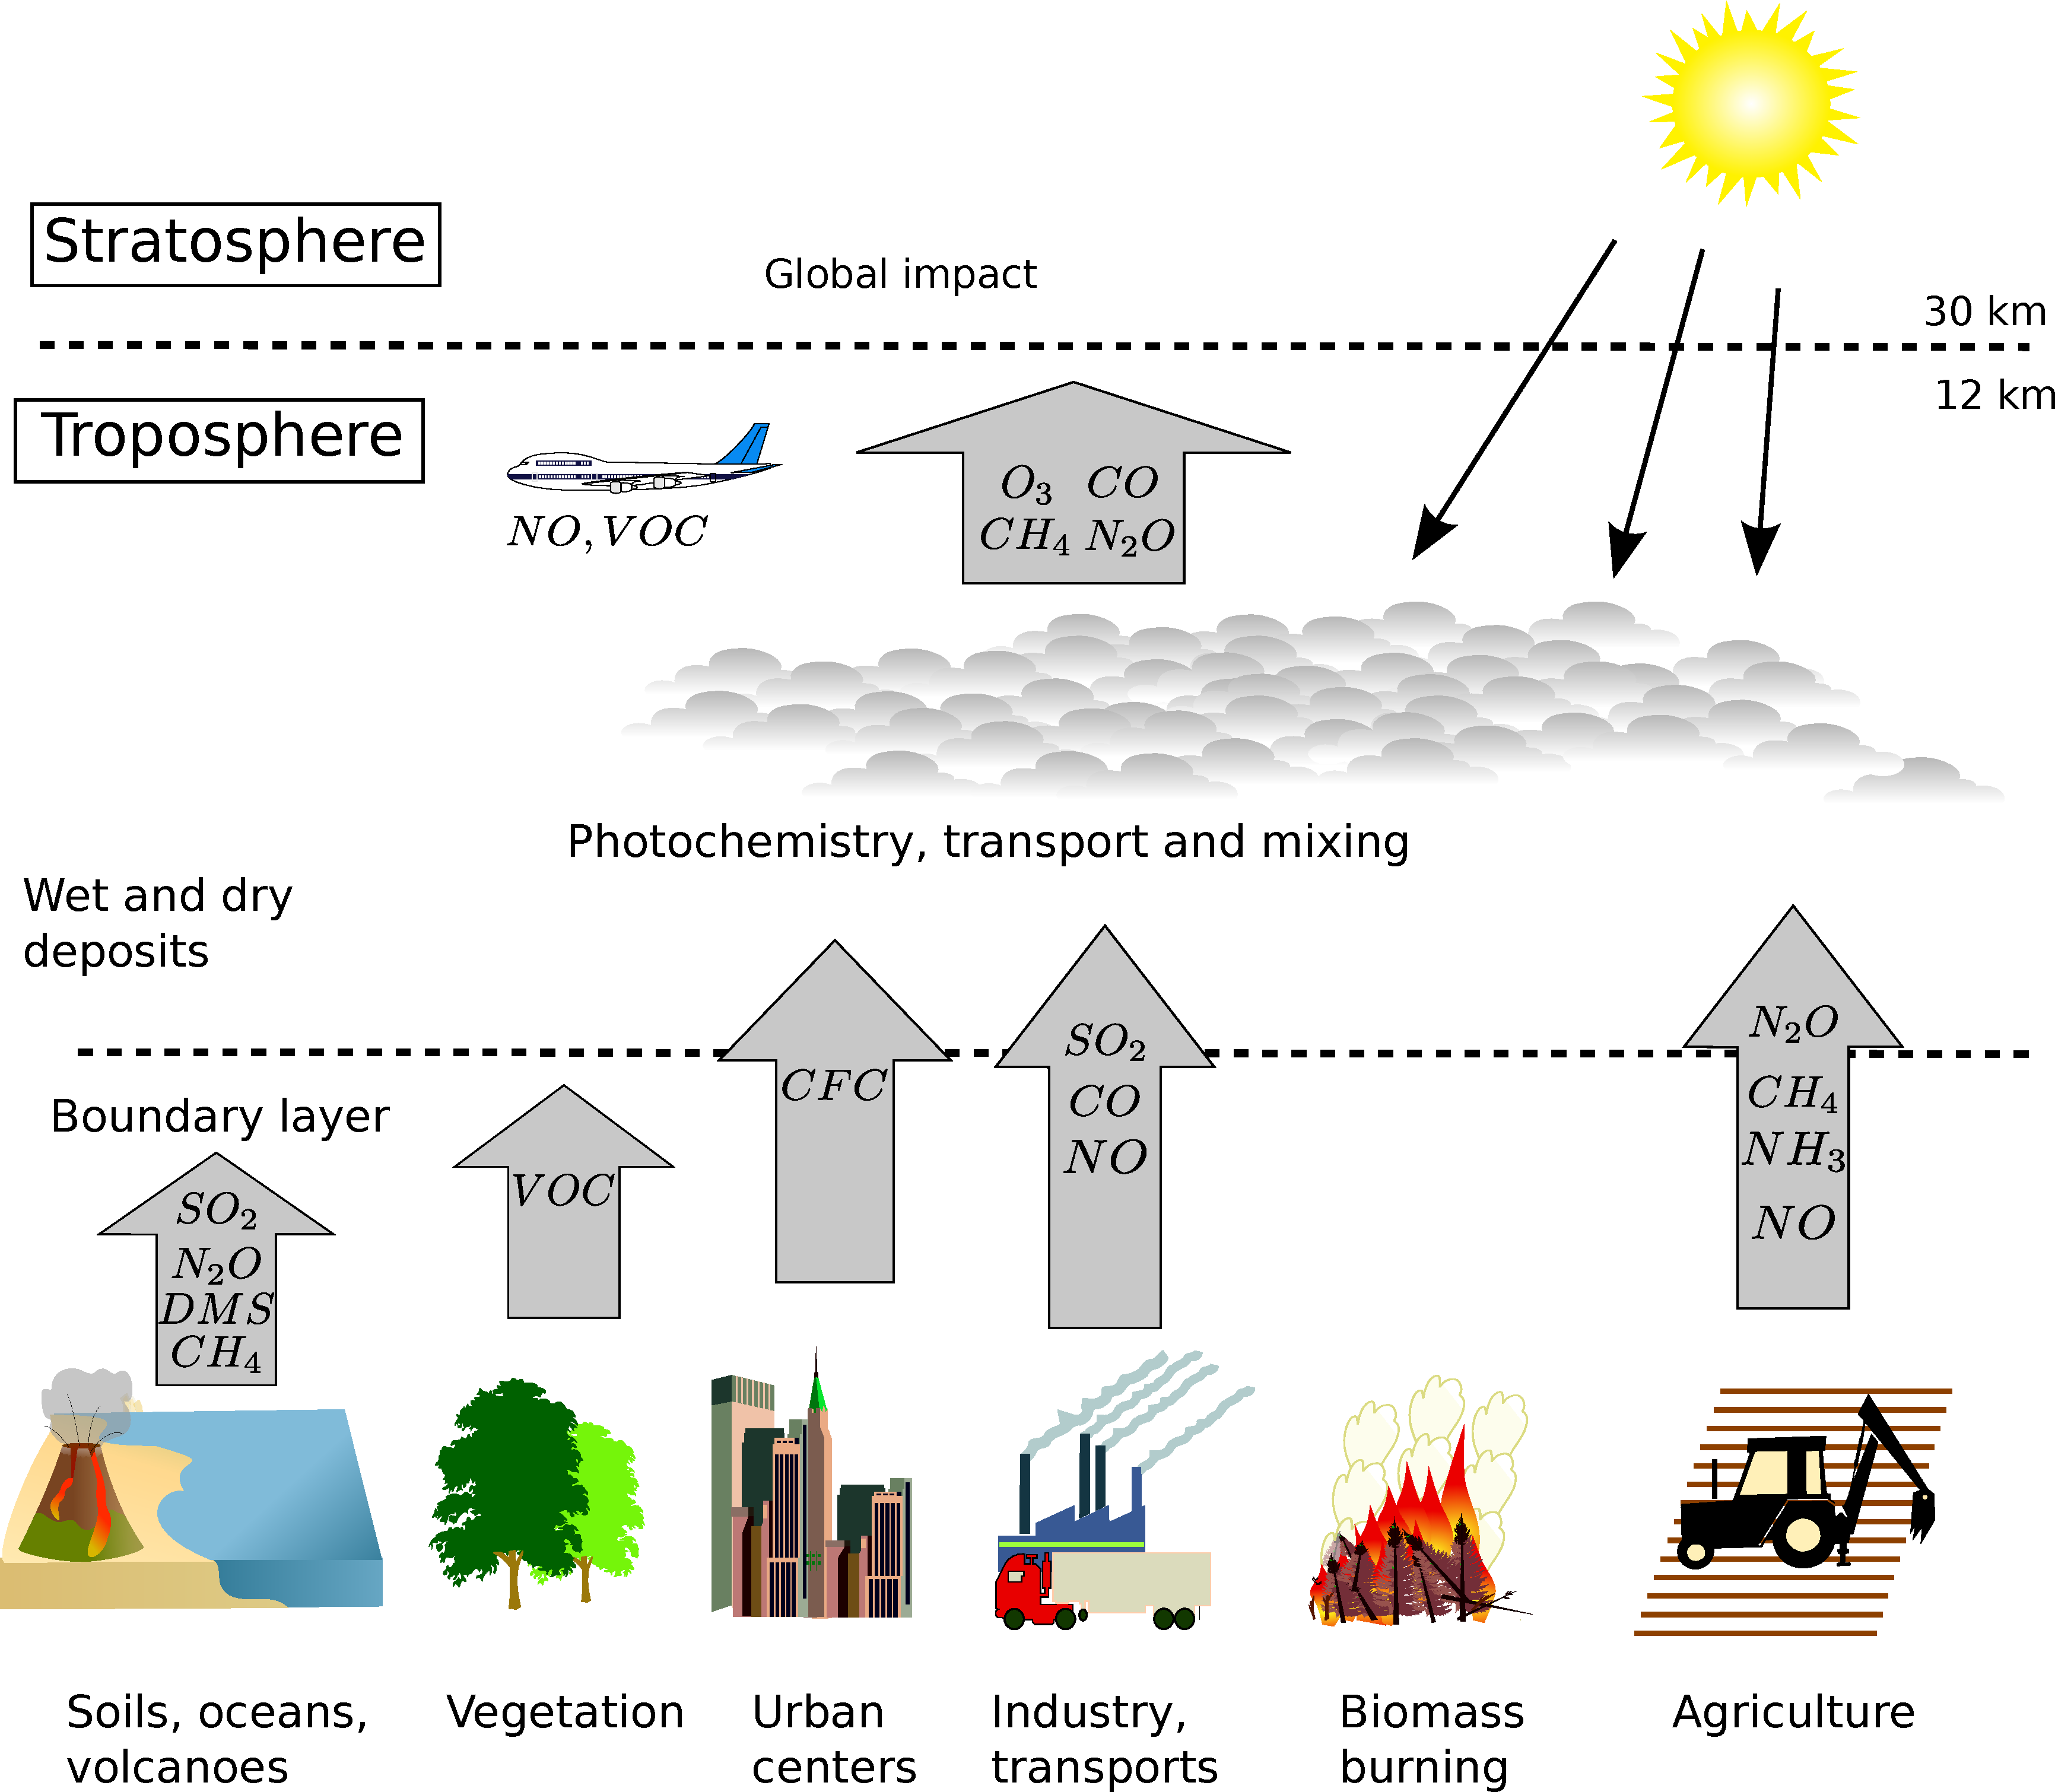
\includegraphics[width=0.8\linewidth]{atmospheric_processes.pdf}
  \caption{Main processes for atmospheric chemistry (inspired from
    \cite{Delmas2005}, with pictures from Wikipedia). VOC stands for Volatile
    Organic Compound, DMS stands for dimethyl sulfide, a biological sulfur
    compound. CFC stands for chlorofluorocarbons, a compound massively used in the
  industry, which contributes to ozone depletion. } \label{fig:atmospheric_proc}
\end{figure}
\begin{figure}
  \centering
  \includegraphics[width=0.8\linewidth]{chemistry_processes.pdf}
  \caption{Main processes involved in the evolution of the chemical
    concentrations (either gaz or particles). They should be represented, at
    least minimally, in a model of the physics and chemistry of the atmosphere
    (inspired from \cite{Delmas2005}). }
  \label{fig:chem_processes}
\end{figure}
CTMs have various applications, such as the estimation of the impact of
anthropogenic emissions. When pollutants are emitted in Asia, like in the
Fukushima Daiichi incident, it can be crucial to model the transport over the
Pacific Ocean. They are also used to study biochemical cycles, such as the
formation or transport of sulfate aerosol particles from volcanic eruptions such
as the eruption of Eyjafjallaj\"okull. They can be used to run paleochemical
simulations of air quality in prehistoric times to evaluate the impact on
chemistry and climate of extreme events like asteroid impacts or volcanic
eruptions. Another active field of CTMs is "chemical weather" forecasting,
where the composition of atmosphere is forecast for several days using weather
forecasts and emissions inventories. In this case, the focus is on the
boundary layer, \gls{stratosphere} and \gls{troposphere} and can be used to
predict the UV index or peaks of pollution. Several countries in Europe are
implementing such systems.  The French government initiated the "Prev'air"
system to offer air quality forecasts for the current day and up to two days
using the MOCAGE and CHIMERE models.  The results are publicly available on the
web (\url{www2.prevair.org}).  CTMs can also be used to study the interactions
between chemistry and climate change.  For example the IGAC committee studies,
among other topics, the impact of ozone on climate change or the effect of
aerosols on clouds (\cite{IGAC2006}).

In this thesis, we focus on the advection and chemistry schemes of a CTM. In
particular, this thesis \DIFdelbegin \DIFdel{is not about developing a dynamical core, which goes far
beyond the transport, but to focus instead on single-tracer }\DIFdelend \DIFaddbegin \DIFadd{focuses on developing the foundation of a CTM by focusing
first on multi-tracers }\DIFaddend advection.  Development of numerical methods for
\DIFdelbegin \DIFdel{transport }\DIFdelend \DIFaddbegin \DIFadd{advection }\DIFaddend has been a very active area of research since the 1960s and is still
continuing today. The research falls into two categories: the first deals with
the numerical methods themselves, while the second focuses on adapting these
methods to the spherical geometry of the atmosphere, which possesses unique
features. Usually referred to as the "pole issue", the main issues with the
traditional regular latitude-longitude grids arise from the convergence of
meridians at the pole and the poles are singularities. This strongly impacts
computational performances and has recently led to research alternatives with
more uniform grids. At the moment, there is no perfect combination of an
advection scheme on a spherical grid.\\ The chemistry in a CTM involves tens of
thousands of chemical species. As it is too expensive to consider all of them, a
hundred of them are considered in practice, along with a thousand of chemical
reactions. Mathematically, this results in a \textit{stiff} set of equations,
\textit{i.e.}, where explicit methods are inefficient. On top of that, chemistry
is completely local to each cell of the grid, contrary to advection. These
factors justify in practice a separation of chemistry and advection in a CTM.

The choice of a model is highly dependant on the computer architecture it will
run on. While mathematical models for weather forecast were developed at the
beginning of the 20th century, the first operational weather forecast appeared
in the 1950s. The increase in computation power led to more complex models and
with finer resolutions ever since. These improvements have in turn put a huge
pressure on computational performances. On one hand, increasing resolution is
beneficial to the accuracy of both advection and chemistry and is especially
useful for GCMS, which are aiming now for a regional scale. On the other hand,
NWFs require computational efficiency as the model must finish fast enough to be
able to run several times per day. This pressure has been fed by two revolutions
in computer architectures. The first was the vector processors, which have been
now supplanted by clusters of processors (up to hundred of thousands of cores).
In the current context, using many-cores has also changed the way parallel
performances are envisioned. The current focus is the ability of an application to
handle an increasing number of cores, also known as \textit{scalability}.

\subsection*{Motivation}
Advection schemes in current operational models can be roughly put into two
categories. The first contains efficient models which are not intrinsically
mass-preserving, the family of the semi-Lagrangian models. Their efficiency comes in
particular from the larger time-step than their Eulerian counterparts.
Mass fixers are used in practice to ensure that mass is conserved globally,
without ensuring local conservation. Unfortunately, these fixers  have an
additional computation cost, which is likely to impact parallel performances.
The second category contains conservative grid-point schemes, which are usually
finite-volume schemes. Efficiency is however severely limited due to the "pole
problem", which constraints the time-step.

This thesis aims at addressing these two issues at once by having a conservative
and efficient \DIFdelbegin \DIFdel{CTM}\DIFdelend \DIFaddbegin \DIFadd{model for advection and chemistry}\DIFaddend . On top of that, we require the
model to have an efficient parallel implementation and to anticipate future
development of parallel architectures, mostly by decreasing the memory
footprint. \DIFdelbegin \DIFdel{We also aim at
presenting }\DIFdelend \DIFaddbegin \DIFadd{In a near future, we also aim to develop a fully-flegded CTM as }\DIFaddend an
alternative to MOCAGE, the CTM of M\'et\'eo-France, and to exploit the parallel
architectures of M\'et\'eo-France. Hence, we present Pangolin, a PArallel
implementatioN of a larGe scale multi-dimensiOnaL \DIFdelbegin \DIFdel{model}\DIFdelend \DIFaddbegin \DIFadd{chemIstry-traNsport
scheme}\DIFaddend , which serves as an efficient parallel framework for atmospheric
advection and chemistry.

\subsection*{Overview}
\begin{itemize}
  \item Chapter~\ref{chap:transport} gives an overview of the different
    advection schemes and introduces the finite-volume scheme chosen for this
    thesis. In a second part, we study the different spherical grids available.
    Then we introduce a new quasi-area preserving grid to remove the "pole
    issue" and show how the scheme is implemented on this grid.
  \item Chapter~\ref{chap:testing} examines the performance of the
    our bi-dimensional advection scheme on algebraic test cases. Pangolin is also
    compared to state-of-the-art transport schemes using a recent
    testing-suite.
  \item Chapter~\ref{chap:parallel} presents the parallelization strategy and
    explains how a custom domain-decom\-position algorithm was developed 
    for an efficient parallelization using the message-passing paradigm. The
    performances are validated in parallel for 2D advection. The impact of
    adding the chemistry is estimated and future strategies are also proposed.
  \item Chapter~\ref{chap:real_case} compares and discusses a 2D run of Pangolin
    using isentropic coordinates to a 3D run of MOCAGE to simulate stratospheric
    ozone distribution over a month. A linear ozone scheme is used in both
    models.
\end{itemize}

% Numbering is changed in transport.tex
